% =====================================================================
%  Chapitre 6 : Modeles de donnees
% =====================================================================
\chapter{Les modèles de données}
\label{ch:modeles}

\chapitreresume{Le catalogue a besoin d'une mémoire. Dans ce chapitre, vous
concevez la base de données de \gesibiblio{} avec les modèles Django : auteurs,
catégories, livres, membres et emprunts. Vous découvrez l'ORM, les relations, les
migrations et les requêtes qui remplacent le SQL.}

\begin{objectifs}
\begin{itemize}
  \item Expliquer le rôle d'un modèle et de l'ORM.
  \item Concevoir les relations entre auteurs, livres, catégories, membres et
        emprunts.
  \item Écrire des modèles complets avec champs, options et contraintes.
  \item Choisir le bon type de champ et le bon comportement \code{on\_delete}.
  \item Créer et appliquer des migrations.
  \item Interroger la base avec l'ORM dans le shell Django.
\end{itemize}
\end{objectifs}

\section{Le modèle et l'ORM}

Un \textbf{modèle} Django est une classe Python qui décrit une table de la base de
données. Chaque attribut de classe devient une colonne. Chaque instance devient une
ligne. Django traduit automatiquement les opérations Python en SQL : c'est
l'\textbf{ORM}, pour \emph{Object Relational Mapper}.

\begin{codebox}[python]{Principe de l'ORM}
# Python
livre = Livre.objects.get(slug="le-petit-prince")
print(livre.titre)

# SQL équivalent, exécuté par Django
# SELECT * FROM catalogue_livre WHERE slug = 'le-petit-prince' LIMIT 1;
\end{codebox}

L'ORM apporte trois avantages :
\begin{itemize}
  \item on écrit du Python, pas du SQL spécifique à une base ;
  \item les requêtes sont paramétrées, ce qui protège des injections SQL ;
  \item les relations sont manipulées comme des objets, avec
        \code{livre.auteur} ou \code{auteur.livres.all()}.
\end{itemize}

\begin{retenir}
Un modèle décrit les données et les règles qui les concernent. La vue ne doit pas
connaître le SQL. Elle interroge les modèles, qui centralisent la logique d'accès
aux données.
\end{retenir}

\section{Concevoir la base de données}

Avant d'écrire du code, prenons le temps de dessiner les données.

\begin{figure}[htbp]
\centering
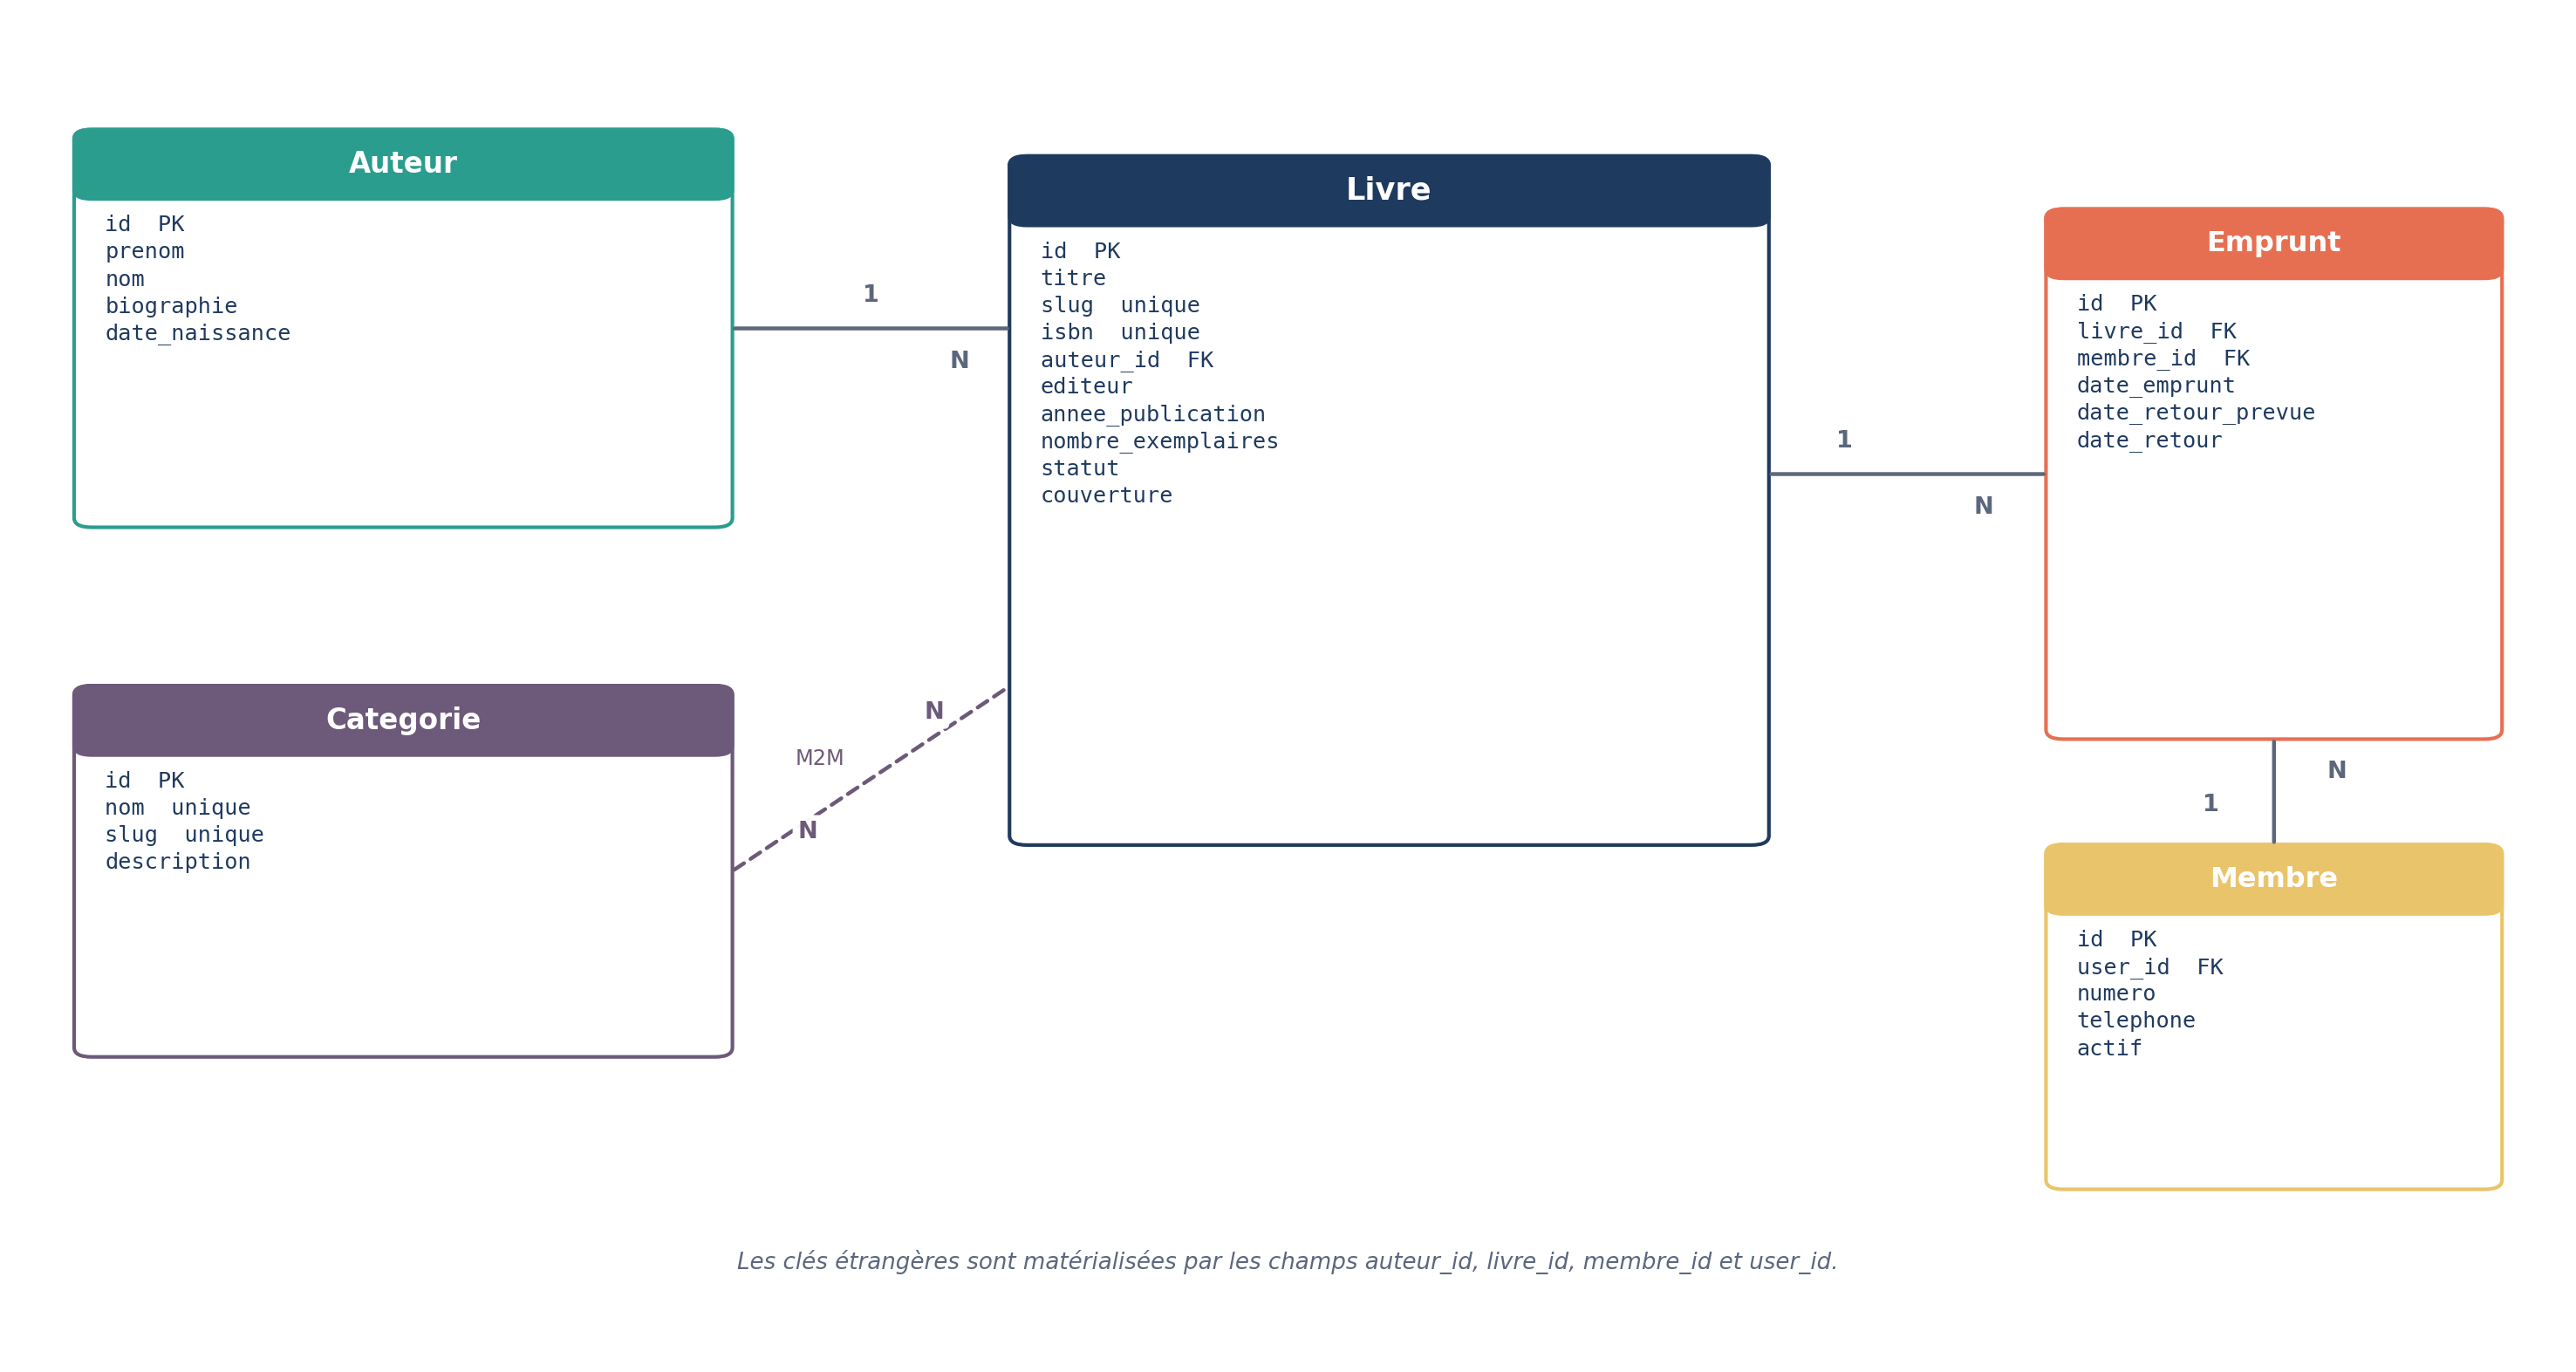
\includegraphics[width=\textwidth]{images/modele_bdd.png}
\caption{Modèle de données de \gesibiblio. Les clés étrangères matérialisent les
relations entre les entités.}
\label{fig:modele-bdd}
\end{figure}

\begin{description}[leftmargin=3.4cm,style=nextline]
  \item[Auteur] Un auteur peut écrire plusieurs livres. Un livre a un seul auteur.
  C'est une relation \og un à plusieurs \fg.
  \item[Catégorie] Un livre peut appartenir à plusieurs catégories, et une
  catégorie contient plusieurs livres. C'est une relation \og plusieurs à
  plusieurs \fg.
  \item[Membre] Un membre est lié à un utilisateur Django par une relation
  \og un à un \fg. Un utilisateur possède au plus un profil de membre.
  \item[Emprunt] Un emprunt relie un livre et un membre. Un livre peut avoir
  plusieurs emprunts dans le temps, un membre aussi.
\end{description}

\begin{note}
Un livre possède un nombre d'exemplaires. Le nombre d'exemplaires disponibles
n'est pas stocké : il se calcule en soustrayant les emprunts en cours. Stocker une
valeur calculable est une source d'incohérence. Nous utiliserons une propriété
Python.
\end{note}

\section{Écrire les modèles}

Ouvrez \code{catalogue/models.py} et remplacez son contenu par le code suivant.
Les commentaires expliquent les choix importants.

\begin{codebox}[python]{catalogue/models.py}
from django.conf import settings
from django.core.validators import (
    MaxValueValidator,
    MinValueValidator,
    RegexValidator,
)
from django.db import models
from django.urls import reverse
from django.utils import timezone


class Categorie(models.Model):
    nom = models.CharField(max_length=80, unique=True)
    slug = models.SlugField(max_length=90, unique=True)
    description = models.TextField(blank=True)

    class Meta:
        ordering = ["nom"]
        verbose_name = "catégorie"
        verbose_name_plural = "catégories"

    def __str__(self):
        return self.nom

    def get_absolute_url(self):
        return reverse(
            "catalogue:categorie_detail",
            kwargs={"slug": self.slug},
        )


class Auteur(models.Model):
    prenom = models.CharField(max_length=80)
    nom = models.CharField(max_length=80)
    biographie = models.TextField(blank=True)
    date_naissance = models.DateField(null=True, blank=True)

    class Meta:
        ordering = ["nom", "prenom"]
        verbose_name = "auteur"
        verbose_name_plural = "auteurs"
        constraints = [
            models.UniqueConstraint(
                fields=["nom", "prenom"],
                name="auteur_unique_nom_prenom",
            ),
        ]

    def __str__(self):
        return f"{self.prenom} {self.nom}"

    @property
    def nom_complet(self):
        return f"{self.prenom} {self.nom}"


class Livre(models.Model):
    class Statut(models.TextChoices):
        DISPONIBLE = "disponible", "Disponible"
        EMPRUNTE = "emprunte", "Emprunté"
        RESERVE = "reserve", "Réservé"
        PERDU = "perdu", "Perdu"

    titre = models.CharField(max_length=200)
    sous_titre = models.CharField(max_length=200, blank=True)
    slug = models.SlugField(max_length=220, unique=True)
    isbn = models.CharField(
        max_length=13,
        unique=True,
        validators=[
            RegexValidator(
                r"^\d{13}$",
                "L'ISBN doit contenir exactement 13 chiffres.",
            ),
        ],
    )
    auteur = models.ForeignKey(
        Auteur,
        on_delete=models.PROTECT,
        related_name="livres",
    )
    categories = models.ManyToManyField(
        Categorie,
        related_name="livres",
        blank=True,
    )
    editeur = models.CharField(max_length=120, blank=True)
    annee_publication = models.PositiveIntegerField(
        validators=[
            MinValueValidator(1450),
            MaxValueValidator(2100),
        ],
    )
    nombre_exemplaires = models.PositiveIntegerField(default=1)
    couverture = models.ImageField(
        upload_to="couvertures/",
        blank=True,
        null=True,
    )
    resume = models.TextField(blank=True)
    statut = models.CharField(
        max_length=20,
        choices=Statut.choices,
        default=Statut.DISPONIBLE,
    )
    cree_le = models.DateTimeField(auto_now_add=True)
    modifie_le = models.DateTimeField(auto_now=True)

    class Meta:
        ordering = ["titre"]
        verbose_name = "livre"
        verbose_name_plural = "livres"
        indexes = [
            models.Index(fields=["titre"]),
        ]

    def __str__(self):
        return self.titre

    def get_absolute_url(self):
        return reverse(
            "catalogue:livre_detail",
            kwargs={"slug": self.slug},
        )

    @property
    def exemplaires_disponibles(self):
        emprunts_en_cours = self.emprunts.filter(
            date_retour__isnull=True
        ).count()
        return max(self.nombre_exemplaires - emprunts_en_cours, 0)

    @property
    def est_disponible(self):
        return (
            self.statut == self.Statut.DISPONIBLE
            and self.exemplaires_disponibles > 0
        )


class Membre(models.Model):
    user = models.OneToOneField(
        settings.AUTH_USER_MODEL,
        on_delete=models.CASCADE,
        related_name="membre",
    )
    numero = models.CharField(max_length=12, unique=True)
    telephone = models.CharField(max_length=20, blank=True)
    adresse = models.CharField(max_length=255, blank=True)
    date_inscription = models.DateField(auto_now_add=True)
    actif = models.BooleanField(default=True)

    class Meta:
        ordering = ["numero"]
        verbose_name = "membre"
        verbose_name_plural = "membres"

    def __str__(self):
        nom = self.user.get_full_name() or self.user.username
        return f"{nom} ({self.numero})"


class Emprunt(models.Model):
    livre = models.ForeignKey(
        Livre,
        on_delete=models.PROTECT,
        related_name="emprunts",
    )
    membre = models.ForeignKey(
        Membre,
        on_delete=models.PROTECT,
        related_name="emprunts",
    )
    date_emprunt = models.DateField(default=timezone.localdate)
    date_retour_prevue = models.DateField()
    date_retour = models.DateField(null=True, blank=True)
    remarque = models.TextField(blank=True)

    class Meta:
        ordering = ["-date_emprunt"]
        verbose_name = "emprunt"
        verbose_name_plural = "emprunts"
        constraints = [
            models.CheckConstraint(
                condition=models.Q(
                    date_retour_prevue__gte=models.F("date_emprunt")
                ),
                name="emprunt_retour_apres_emprunt",
            ),
        ]

    def __str__(self):
        return f"{self.livre} -> {self.membre}"

    @property
    def est_en_retard(self):
        if self.date_retour:
            return False
        return self.date_retour_prevue < timezone.localdate()

    @property
    def duree_retard(self):
        if not self.est_en_retard:
            return 0
        return (timezone.localdate() - self.date_retour_prevue).days
\end{codebox}

\begin{attention}
La contrainte \code{CheckConstraint} utilise l'argument \code{condition} à partir
de Django 5.1. Avec Django 5.0 et les versions précédentes, l'argument s'appelle
\code{check}. Si vous utilisez une version plus ancienne, adaptez cette ligne.
\end{attention}

\section{Les types de champs}

\begin{table}[htbp]
\centering
\small
\begin{tabularx}{\textwidth}{L{4.3cm} X}
\toprule
\textbf{Champ} & \textbf{Usage} \\
\midrule
\code{CharField} & Chaîne courte. Obligatoire : \code{max\_length}. \\
\code{TextField} & Texte long, sans limite de taille pratique. \\
\code{SlugField} & Chaîne compatible avec une URL : lettres, chiffres, tirets. \\
\code{EmailField} & Adresse électronique validée. \\
\code{URLField} & URL validée. \\
\code{IntegerField} & Entier positif ou négatif. \\
\code{PositiveIntegerField} & Entier positif ou nul. \\
\code{DecimalField} & Nombre décimal exact. Obligatoire :
\code{max\_digits}, \code{decimal\_places}. \\
\code{BooleanField} & Vrai ou faux. \\
\code{DateField} & Date. \code{auto\_now\_add} à la création,
\code{auto\_now} à chaque sauvegarde. \\
\code{DateTimeField} & Date et heure. \\
\code{ImageField} & Image. Nécessite Pillow. \\
\code{FileField} & Fichier quelconque. \\
\code{ForeignKey} & Relation un à plusieurs. \\
\code{ManyToManyField} & Relation plusieurs à plusieurs. \\
\code{OneToOneField} & Relation un à un. \\
\code{JSONField} & Données JSON structurées. \\
\bottomrule
\end{tabularx}
\caption{Les types de champs les plus utilisés.}
\end{table}

\subsection{null ou blank ?}

\begin{description}[leftmargin=2.7cm,style=nextline]
  \item[\code{null=True}] Autorise la valeur \code{NULL} dans la base. À réserver
  aux champs non textuels : dates, nombres, relations.
  \item[\code{blank=True}] Autorise une valeur vide dans les formulaires. Pour un
  \code{CharField}, la valeur enregistrée est une chaîne vide, pas \code{NULL}.
\end{description}

\begin{bonne}
Pour un \code{CharField} ou un \code{TextField}, utilisez \code{blank=True} sans
\code{null=True}. Sinon, vous aurez deux représentations du vide : \code{NULL} et
\code{""}. Pour un \code{DateField} ou une \code{ForeignKey} optionnelle, utilisez
les deux.
\end{bonne}

\subsection{Les choix avec TextChoices}

\code{Livre.Statut} est une classe imbriquée qui hérite de \code{models.TextChoices}.
Elle associe une valeur stockée en base à un libellé affiché :

\begin{codebox}[python]{Utilisation des choix}
livre.statut = Livre.Statut.EMPRUNTE
livre.get_statut_display()   # "Emprunté"
\end{codebox}

\begin{bonne}
Utilisez \code{TextChoices} plutôt qu'une liste de tuples. Le code devient plus
lisible, les valeurs sont centralisées et les libellés sont traduisibles.
\end{bonne}

\section{Les relations et on\_delete}

\subsection{ForeignKey}

\begin{codebox}[python]{Relation un à plusieurs}
auteur = models.ForeignKey(
    Auteur,
    on_delete=models.PROTECT,
    related_name="livres",
)
\end{codebox}

\begin{itemize}
  \item \code{livre.auteur} renvoie l'objet \code{Auteur}.
  \item \code{auteur.livres.all()} renvoie les livres de cet auteur.
  \item \code{related\_name} remplace le nom par défaut \code{livre\_set}. Il rend
        le code plus lisible.
\end{itemize}

\subsection{ManyToManyField}

\begin{codebox}[python]{Relation plusieurs à plusieurs}
categories = models.ManyToManyField(
    Categorie,
    related_name="livres",
    blank=True,
)
\end{codebox}

Django crée une table intermédiaire. La méthode \code{add} associe une catégorie
à un livre, et \code{livre.categories.all()} renvoie ses catégories.

\subsection{OneToOneField}

\begin{codebox}[python]{Relation un à un}
user = models.OneToOneField(
    settings.AUTH_USER_MODEL,
    on_delete=models.CASCADE,
    related_name="membre",
)
\end{codebox}

Chaque utilisateur possède au plus un profil \code{Membre}. On accède au profil
avec \code{request.user.membre}. Attention : si le profil n'existe pas, l'accès
lève une exception \code{RelatedObjectDoesNotExist}. Nous le créerons
automatiquement à l'inscription.

\subsection{Les comportements on\_delete}

\begin{table}[htbp]
\centering
\small
\begin{tabularx}{\textwidth}{L{3.4cm} X}
\toprule
\textbf{Valeur} & \textbf{Comportement} \\
\midrule
\code{CASCADE} & Supprime aussi les objets liés. \\
\code{PROTECT} & Empêche la suppression tant qu'un objet lié existe. \\
\code{RESTRICT} & Empêche la suppression, avec une erreur plus récente que
\code{PROTECT}. \\
\code{SET\_NULL} & Met la clé étrangère à \code{NULL}. Nécessite
\code{null=True}. \\
\code{SET\_DEFAULT} & Met la valeur par défaut. \\
\code{DO\_NOTHING} & Ne fait rien. Risque d'incohérence, à éviter. \\
\bottomrule
\end{tabularx}
\caption{Comportements possibles lors de la suppression d'un objet lié.}
\end{table}

\begin{bonne}
Pour un catalogue, \code{PROTECT} est souvent le bon choix : on ne supprime pas un
auteur qui a encore des livres, ni un livre qui a des emprunts. Pour un profil
utilisateur, \code{CASCADE} est logique : supprimer le compte supprime le profil.
\end{bonne}

\section{Les options Meta et les contraintes}

La classe \code{Meta} configure le modèle :
\begin{itemize}
  \item \code{ordering} : ordre par défaut des requêtes ;
  \item \code{verbose\_name} et \code{verbose\_name\_plural} : libellés dans
        l'administration ;
  \item \code{indexes} : index de base de données ;
  \item \code{constraints} : contraintes d'unicité ou de validation.
\end{itemize}

\begin{codebox}[python]{Meta du modèle Livre}
class Meta:
    ordering = ["titre"]
    indexes = [
        models.Index(fields=["titre"]),
    ]
\end{codebox}

\begin{note}
Un index accélère certaines lectures mais ralentit les écritures et occupe de
l'espace. \code{unique=True} crée déjà un index : inutile d'ajouter
\code{db\_index=True} sur un champ unique. Les recherches \code{icontains} avec
un joker en tête ne profitent pas toujours d'un index classique.
\end{note}

\section{Les méthodes et propriétés}

\subsection{\_\_str\_\_}

\code{\_\_str\_\_} définit l'affichage d'un objet dans l'administration, le shell
et les messages. Sans elle, vous verriez \code{Livre object (1)}.

\begin{codebox}[python]{Exemple}
def __str__(self):
    return self.titre
\end{codebox}

\subsection{get\_absolute\_url}

Cette méthode renvoie l'URL publique de l'objet. Elle est utilisée par
l'administration et par \code{redirect(livre)}.

\begin{codebox}[python]{Exemple}
def get_absolute_url(self):
    return reverse(
        "catalogue:livre_detail",
        kwargs={"slug": self.slug},
    )
\end{codebox}

\subsection{Les propriétés calculées}

\begin{codebox}[python]{Propriétés du modèle Livre}
@property
def exemplaires_disponibles(self):
    emprunts_en_cours = self.emprunts.filter(
        date_retour__isnull=True
    ).count()
    return max(self.nombre_exemplaires - emprunts_en_cours, 0)

@property
def est_disponible(self):
    return (
        self.statut == self.Statut.DISPONIBLE
        and self.exemplaires_disponibles > 0
    )
\end{codebox}

\begin{attention}
Une propriété n'est pas une colonne. Elle est recalculée à chaque accès. Dans une
liste de 100 livres, \code{livre.exemplaires\_disponibles} déclenche jusqu'à 100
requêtes. Pour optimiser, utilisez \code{annotate} et \code{Count} dans la vue.
Nous verrons cette technique avec l'ORM.
\end{attention}

\section{Les migrations}

Une migration est un fichier Python qui décrit une modification du schéma. Django
la génère à partir de vos modèles.

\subsection{Créer la migration}

\begin{terminal}
python manage.py makemigrations catalogue
\end{terminal}

Sortie attendue :

\begin{terminal}
Migrations for 'catalogue':
  catalogue/migrations/0001_initial.py
    + Create model Categorie
    + Create model Auteur
    + Create model Livre
    + Create model Membre
    + Create model Emprunt
\end{terminal}

Le fichier \code{0001\_initial.py} contient les opérations. On peut le lire, mais
on ne le modifie pas à la main après l'avoir appliqué.

\subsection{Inspecter le SQL}

\begin{terminal}
python manage.py sqlmigrate catalogue 0001
\end{terminal}

Vous voyez les ordres \code{CREATE TABLE}, les clés étrangères et les index. C'est
utile pour comprendre ce que Django fait réellement.

\subsection{Appliquer la migration}

\begin{terminal}
python manage.py migrate
\end{terminal}

Sortie :

\begin{terminal}
Operations to perform:
  Apply all migrations: admin, auth, catalogue, contenttypes, sessions
Running migrations:
  Applying catalogue.0001_initial... OK
\end{terminal}

\subsection{Vérifier l'état}

\begin{terminal}
python manage.py showmigrations catalogue
\end{terminal}

\begin{terminal}
catalogue
 [X] 0001_initial
\end{terminal}

La croix indique que la migration est appliquée.

\begin{bonne}
Versionnez toujours le dossier \code{migrations/}. Ne supprimez pas les fichiers
après les avoir appliqués. Pour renommer une migration, utilisez
\code{makemigrations --name} avant de l'appliquer. En production, sauvegardez la
base avant toute migration.
\end{bonne}

\begin{piege}
Si vous modifiez un modèle et que \code{migrate} ne fait rien, c'est que vous avez
oublié \code{makemigrations}. Si \code{makemigrations} ne détecte aucun changement
alors que vous avez modifié le fichier, vérifiez que l'application est bien dans
\code{INSTALLED\_APPS} et que le serveur n'utilise pas un autre fichier.
\end{piege}

\section{Découvrir l'ORM dans le shell}

Ouvrez le shell Django :

\begin{terminal}
python manage.py shell
\end{terminal}

\subsection{Créer des données}

\begin{codebox}[python]{Shell Django}
from catalogue.models import Auteur, Categorie, Livre

auteur = Auteur.objects.create(
    prenom="Antoine",
    nom="Saint-Exupéry",
    biographie="Aviateur et écrivain français.",
)
roman = Categorie.objects.create(nom="Roman", slug="roman")
livre = Livre.objects.create(
    titre="Le Petit Prince",
    slug="le-petit-prince",
    isbn="9782070612758",
    auteur=auteur,
    annee_publication=1943,
    nombre_exemplaires=3,
    resume="Un aviateur rencontre un petit prince.",
)
livre.categories.add(roman)
livre
\end{codebox}

L'affichage de \code{livre} utilise \code{\_\_str\_\_} et renvoie
\code{<Livre: Le Petit Prince>}.

\subsection{Lire des données}

\begin{codebox}[python]{Requêtes de base}
Livre.objects.count()
Livre.objects.all()
Livre.objects.get(slug="le-petit-prince")
Livre.objects.filter(titre__icontains="prince")
Livre.objects.exclude(statut="perdu")
Livre.objects.filter(annee_publication__gte=1900)
Livre.objects.filter(auteur__nom="Camus")
Livre.objects.order_by("titre")
Livre.objects.values_list("titre", flat=True)
Livre.objects.exists()
\end{codebox}

\begin{description}[leftmargin=4.2cm,style=nextline]
  \item[\code{get()}] Renvoie un objet et un seul. Lève \code{DoesNotExist} si
  aucun objet ne correspond, \code{MultipleObjectsReturned} si plusieurs.
  \item[\code{filter()}] Renvoie un \code{QuerySet}, même vide.
  \item[\code{icontains}] Recherche insensible à la casse.
  \item[\code{gte}] Supérieur ou égal. Autres suffixes : \code{gt}, \code{lt},
  \code{lte}, \code{startswith}, \code{endswith}, \code{in}.
\end{description}

\subsection{Les objets Q et F}

\code{Q} combine des conditions avec \code{|} (ou) et \code{\&} (et) :

\begin{codebox}[python]{Conditions complexes}
from django.db.models import Q

Livre.objects.filter(
    Q(titre__icontains="prince") | Q(isbn__icontains="978")
)
\end{codebox}

\code{F} référence un champ dans la requête, sans le charger en Python :

\begin{codebox}[python]{Expression F}
from django.db.models import F

Livre.objects.filter(
    nombre_exemplaires__gt=1
).update(nombre_exemplaires=F("nombre_exemplaires") + 1)
\end{codebox}

\begin{attention}
\code{update()} modifie directement en base et ne déclenche pas les méthodes
\code{save()} des modèles. Les signaux \code{pre\_save} et \code{post\_save} ne
sont pas exécutés. Utilisez-le pour des mises à jour de masse, pas pour une
logique métier complexe.
\end{attention}

\subsection{select\_related et prefetch\_related}

Le problème N+1 se produit lorsqu'une boucle déclenche une requête par élément :

\begin{codebox}[python]{Problème N+1}
for livre in Livre.objects.all():
    print(livre.auteur.nom)   # une requête par livre
\end{codebox}

Pour une clé étrangère, utilisez \code{select\_related} :

\begin{codebox}[python]{Requête optimisée}
for livre in Livre.objects.select_related("auteur"):
    print(livre.auteur.nom)   # une seule requête
\end{codebox}

Pour une relation plusieurs à plusieurs ou une relation inverse, utilisez
\code{prefetch\_related} :

\begin{codebox}[python]{Prefetch}
for livre in Livre.objects.prefetch_related("categories"):
    for categorie in livre.categories.all():
        print(categorie.nom)
\end{codebox}

\begin{bonne}
\code{select\_related} fait une jointure SQL et convient aux clés étrangères et
aux relations un à un. \code{prefetch\_related} exécute une requête séparée et
convient aux relations plusieurs à plusieurs et aux relations inverses.
\end{bonne}

\subsection{Agrégations et annotations}

\begin{codebox}[python]{Compter et agréger}
from django.db.models import Count, Avg

Livre.objects.aggregate(total=Count("id"))
Categorie.objects.annotate(nb_livres=Count("livres"))
\end{codebox}

\code{aggregate} renvoie un dictionnaire pour l'ensemble du QuerySet.
\code{annotate} ajoute un attribut calculé à chaque objet.

\section{Exercices}

\begin{exercice}[ : ajouter un champ]
Ajoutez un champ \code{nombre\_pages} au modèle \code{Livre}, de type
\code{PositiveIntegerField}, avec une valeur par défaut de 0. Créez et appliquez
la migration.
\end{exercice}

\begin{correction}
\begin{codebox}[python]{catalogue/models.py, extrait}
nombre_pages = models.PositiveIntegerField(default=0)
\end{codebox}

\begin{terminal}
python manage.py makemigrations catalogue --name ajout_nombre_pages
python manage.py migrate
\end{terminal}

La valeur par défaut évite le message interactif de Django pour les lignes
existantes. En production, une valeur par défaut explicite est souvent préférable
à une valeur temporaire.
\end{correction}

\begin{exercice}[ : ajouter un modèle Langue]
Créez un modèle \code{Langue} avec \code{nom} et \code{code}. Ajoutez une clé
étrangère optionnelle \code{langue} au modèle \code{Livre}, avec
\code{on\_delete=models.SET\_NULL}. Générez la migration.
\end{exercice}

\begin{correction}
\begin{codebox}[python]{catalogue/models.py, extrait}
class Langue(models.Model):
    nom = models.CharField(max_length=60, unique=True)
    code = models.CharField(max_length=5, unique=True)

    class Meta:
        ordering = ["nom"]

    def __str__(self):
        return self.nom


class Livre(models.Model):
    # ... champs existants
    langue = models.ForeignKey(
        Langue,
        on_delete=models.SET_NULL,
        null=True,
        blank=True,
        related_name="livres",
    )
\end{codebox}

\begin{terminal}
python manage.py makemigrations catalogue --name ajout_langue
python manage.py migrate
\end{terminal}

\code{SET\_NULL} exige \code{null=True}. Sans cela, Django refuse la migration ou
provoque une erreur à la suppression d'une langue liée.
\end{correction}

\begin{exercice}[ : requêtes]
Dans le shell, trouvez :
\begin{enumerate}
  \item tous les livres publiés après 1950 ;
  \item le nombre de livres de la catégorie \og Roman \fg ;
  \item les livres dont le titre contient \og prince \fg, triés par année ;
  \item l'auteur du livre \og Le Petit Prince \fg.
\end{enumerate}
\end{exercice}

\begin{correction}
\begin{codebox}[python]{Shell Django}
from catalogue.models import Categorie, Livre

Livre.objects.filter(annee_publication__gt=1950)
Categorie.objects.get(slug="roman").livres.count()
Livre.objects.filter(
    titre__icontains="prince"
).order_by("annee_publication")
Livre.objects.get(slug="le-petit-prince").auteur
\end{codebox}

La dernière expression renvoie l'objet \code{Auteur} grâce à la clé étrangère.
Django exécute une requête supplémentaire si l'auteur n'a pas été chargé avec
\code{select\_related}.
\end{correction}

\begin{retenir}
\begin{itemize}
  \item Un modèle décrit une table ; l'ORM traduit Python en SQL.
  \item \code{ForeignKey}, \code{ManyToManyField} et \code{OneToOneField} couvrent
        les relations.
  \item \code{on\_delete=PROTECT} protège les données liées.
  \item \code{makemigrations} prépare, \code{migrate} applique.
  \item \code{get}, \code{filter}, \code{exclude} et \code{order\_by} forment la
        base des requêtes.
  \item \code{select\_related} et \code{prefetch\_related} évitent le problème
        N+1.
\end{itemize}
\end{retenir}
